\section{Sprint 3 - Summary}

During sprint 3, four variable pitch mechanisms were assembled with Align T-rex 500 RC helicopter tail mechanisms and the 880KV 3DR motors.(Fig. \ref{fig:before} \& \ref{fig:after} )

\begin{figure}[h]
        \centering
         \begin{minipage}[b]{0.4\textwidth}
            \includegraphics[width = 1\textwidth]{VAPIQ-PICTURES/BeforeAssembly.jpg}
              \caption{Variable Pitch Parts}
            \label{fig:before}
        \end{minipage}
        \hfill
        \begin{minipage}[b]{0.4\textwidth}
            \includegraphics[width = 0.7\textwidth]{VAPIQ-PICTURES/AfterAssemblyVPQ.jpg}
            \caption{Variable Pitch Assembly}
            \label{fig:after}
        \end{minipage}
\end{figure}

The motors from 3DR with 880 KV were mounted straight under the mechanism and a symmetric airfoil capable of generating equal amounts of thrust in each direction was added. The mechanisms function and rotation worked perfectly, but each full assembly with motors, ESC`s, propellers, servos, servo mounts, linkage rods and carbon tubes, weighed approximately 250 g each. To build a sufficiently functioning quadcopter, thrust to weight ratio should be at least 2:1 as a rule of thumb. Since this is a custom build, it was hard to estimate what lift we could achieve with this motor-propeller assembly theoretically, therefore the team built a simple thrust test rig which could measure the actual thrust produced by the motors (Fig. \ref{fig:testrig} \& \ref{fig:testrigf2}). 

\begin{figure}[h]
        \centering
         \begin{minipage}[b]{0.4\textwidth}
            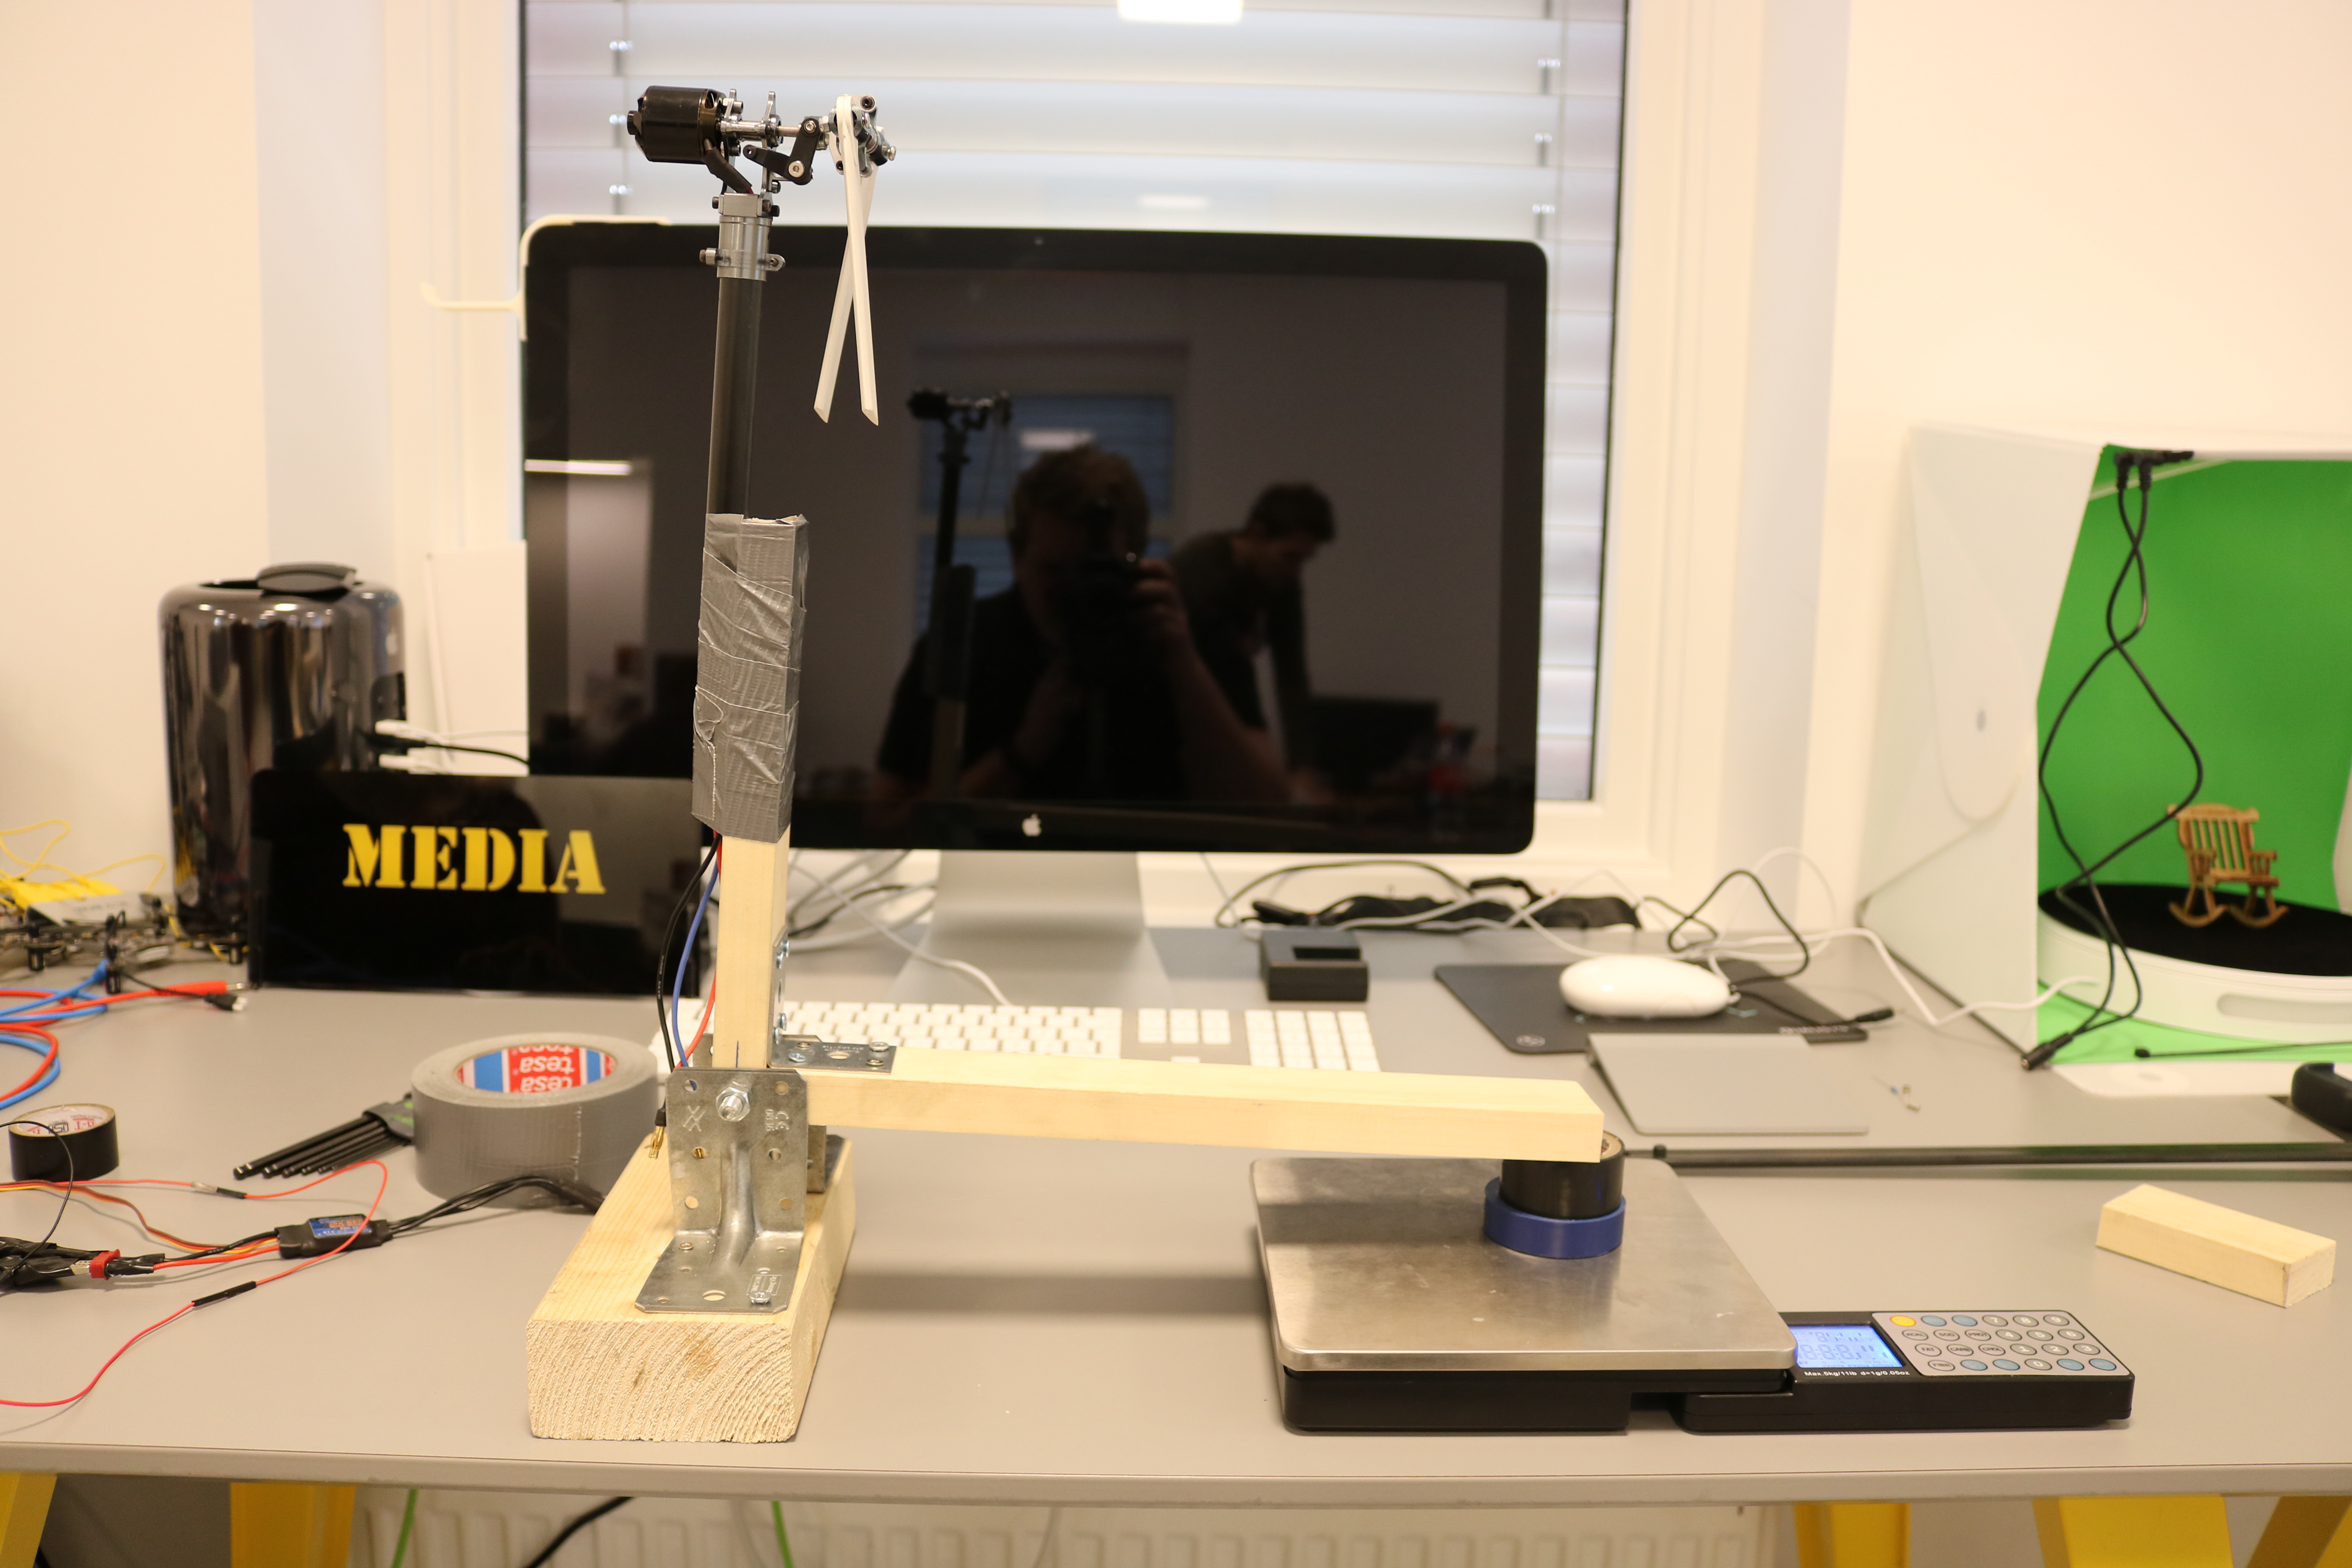
\includegraphics[width = 1\textwidth]{VAPIQ-PICTURES/VPQtestRig}
              \caption{Thrust Test Rig}
            \label{fig:testrig}
        \end{minipage}
        \hfill
        \begin{minipage}[b]{0.4\textwidth}
            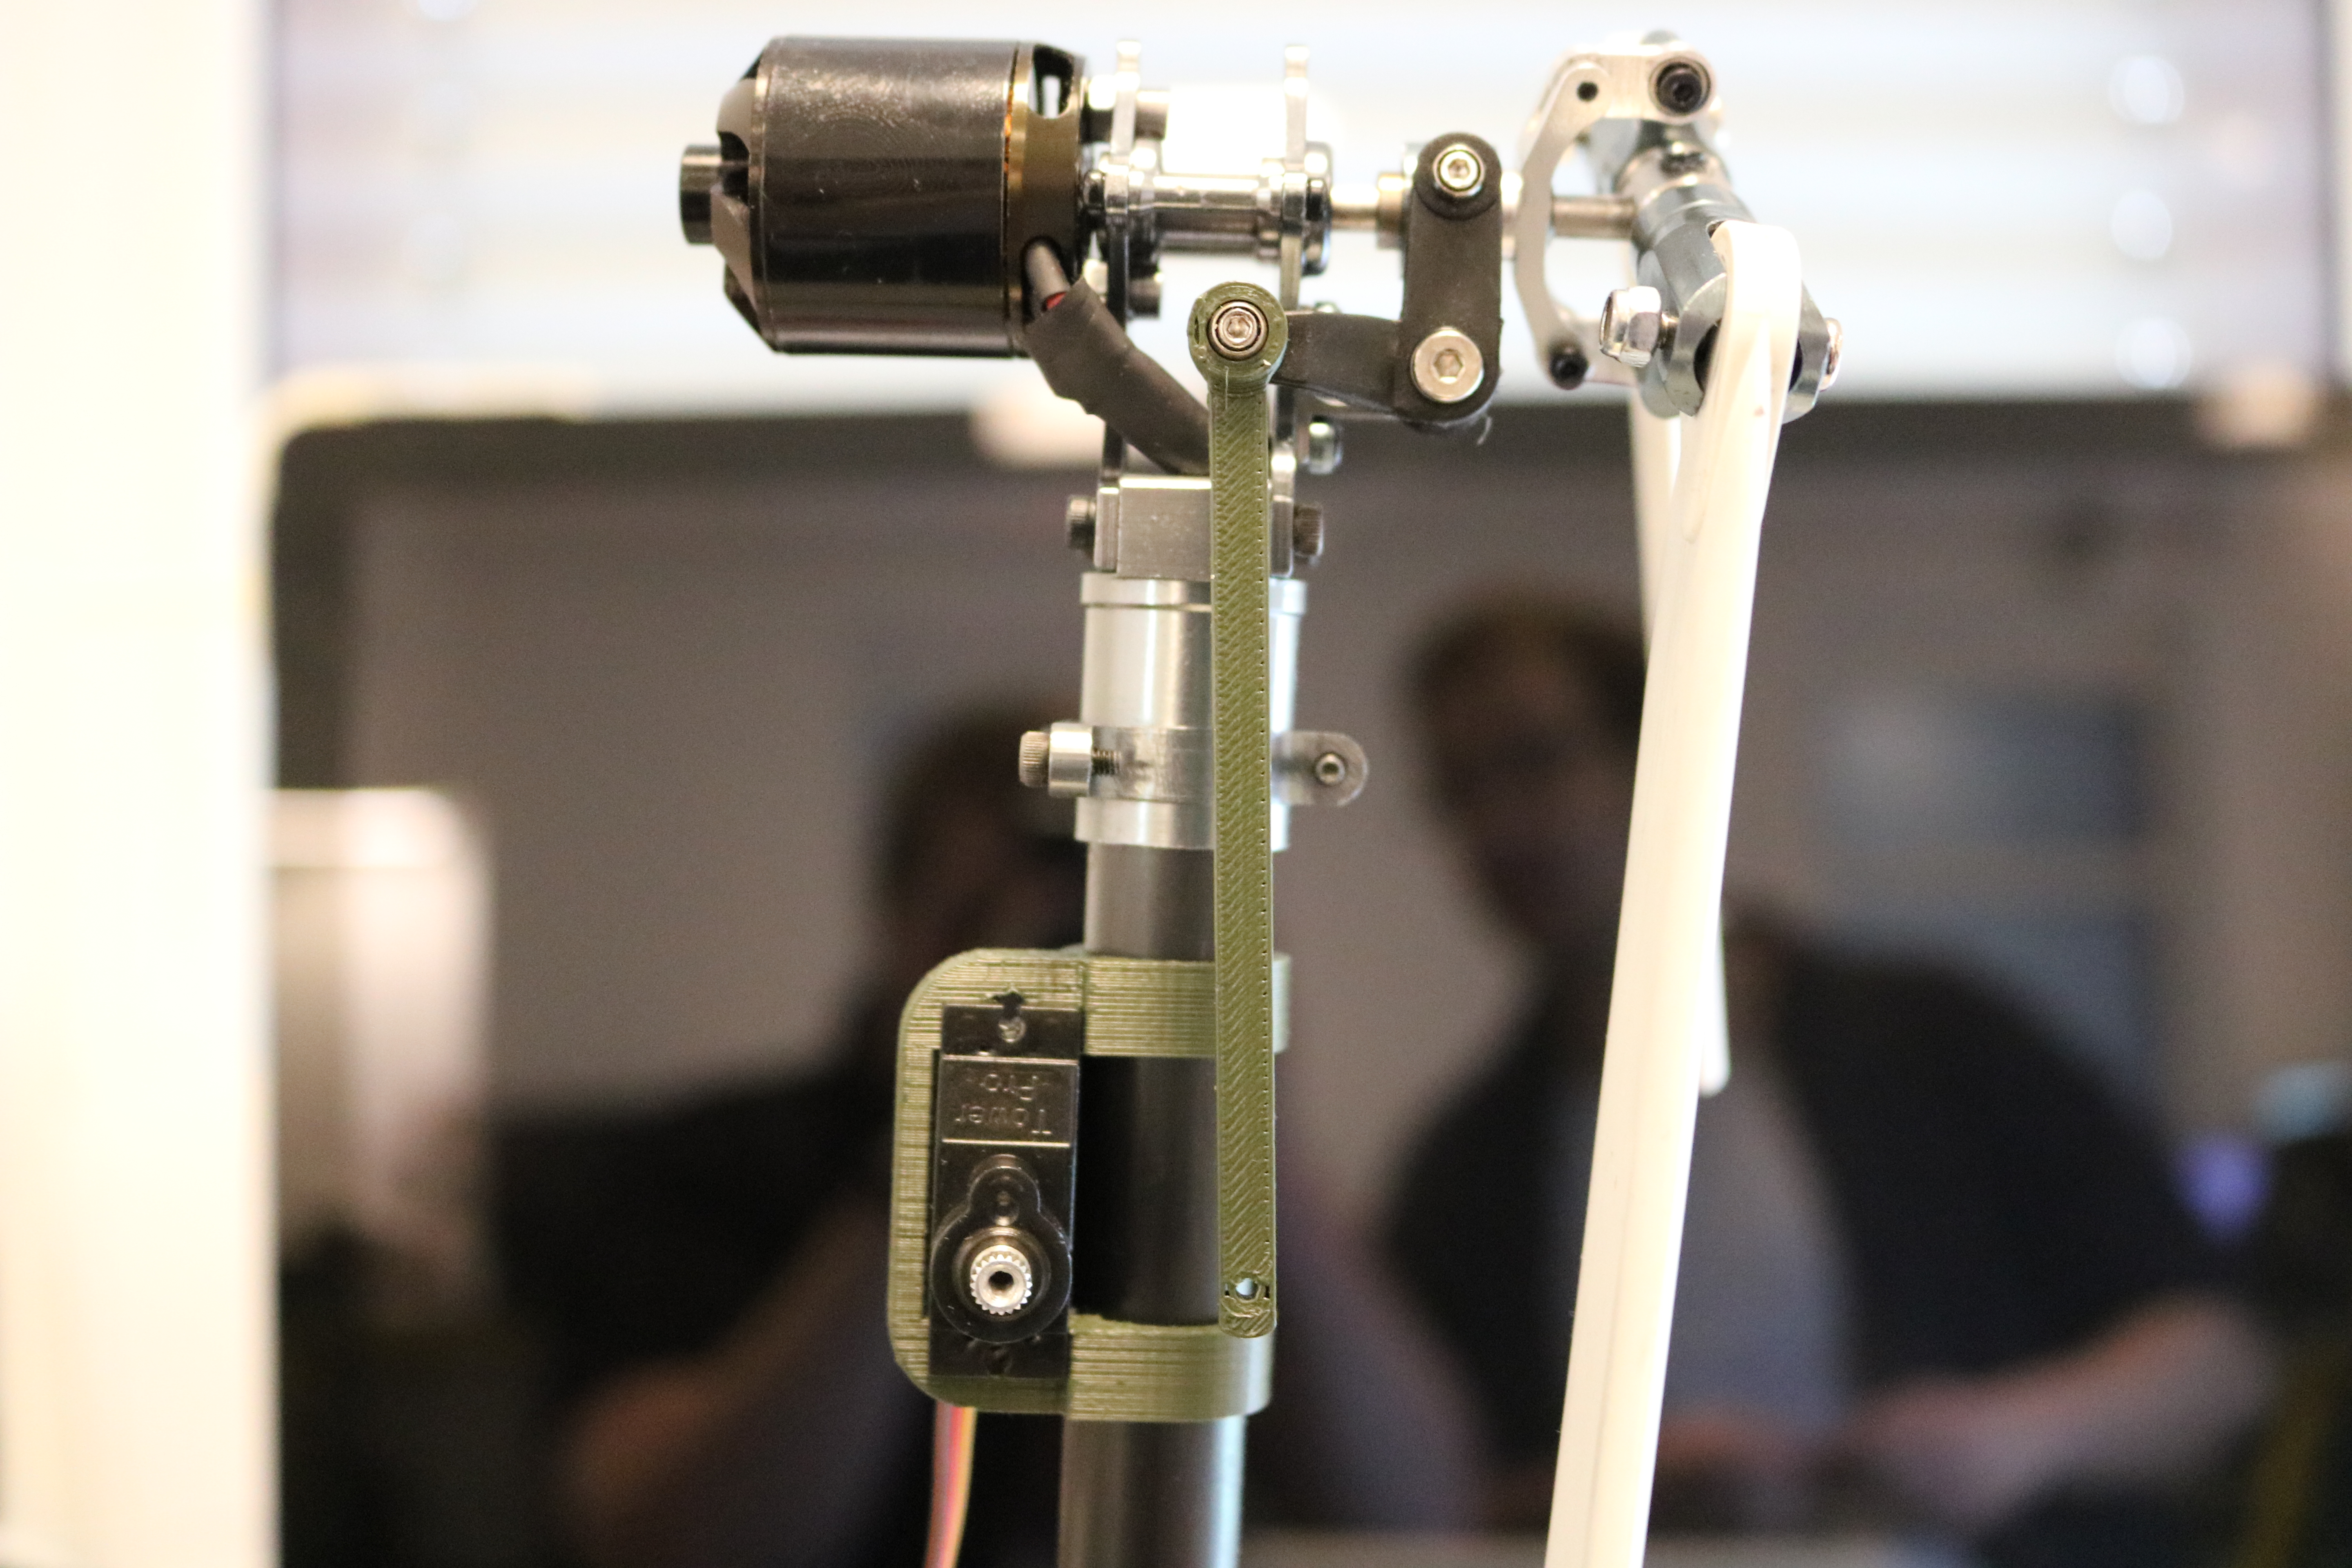
\includegraphics[width = 1\textwidth]{VAPIQ-PICTURES/VpMechanism}
            \caption{Variable Pitch Assembly With Servo}
            \label{fig:testrig2}
        \end{minipage}
\end{figure}


The measured thrust of the motors was approximately 500 g with 3 cell battery voltage, and 700 g with four cell voltage. This adds up to a maximum thrust of 2,4 kg, while the mass budget for this quadcopter was about 1800g. The problem was that with four cell voltage and max speed, the motors started to overheat and consumed a lot of power (18,6 Amps on one motor). On the basis of this information, it is not very plausible that this assembly would yield enough lift for the quadcopter. \\
\\
In sprint 3, the team established P-control in the test rig about one axis (Fig. \ref{fig:oneaxis}). The team also established bluetooth communication with Qualisys. Design wise, there has been generated concepts for fixed pitch. A new design plan for the variable pitch quadcopter had to be made. The team also investigated several other options for the flight controller. This includes planning our own setup as well as looking into the possibility of modifying ArduPilotMega or other existing platforms. The biggest problem of using existing flight controllers is the shear amount of code and interdependencies, and the fact that no open-source controller on the market has functionality that supports variable pitch. 

\begin{figure}[h]
        \centering
        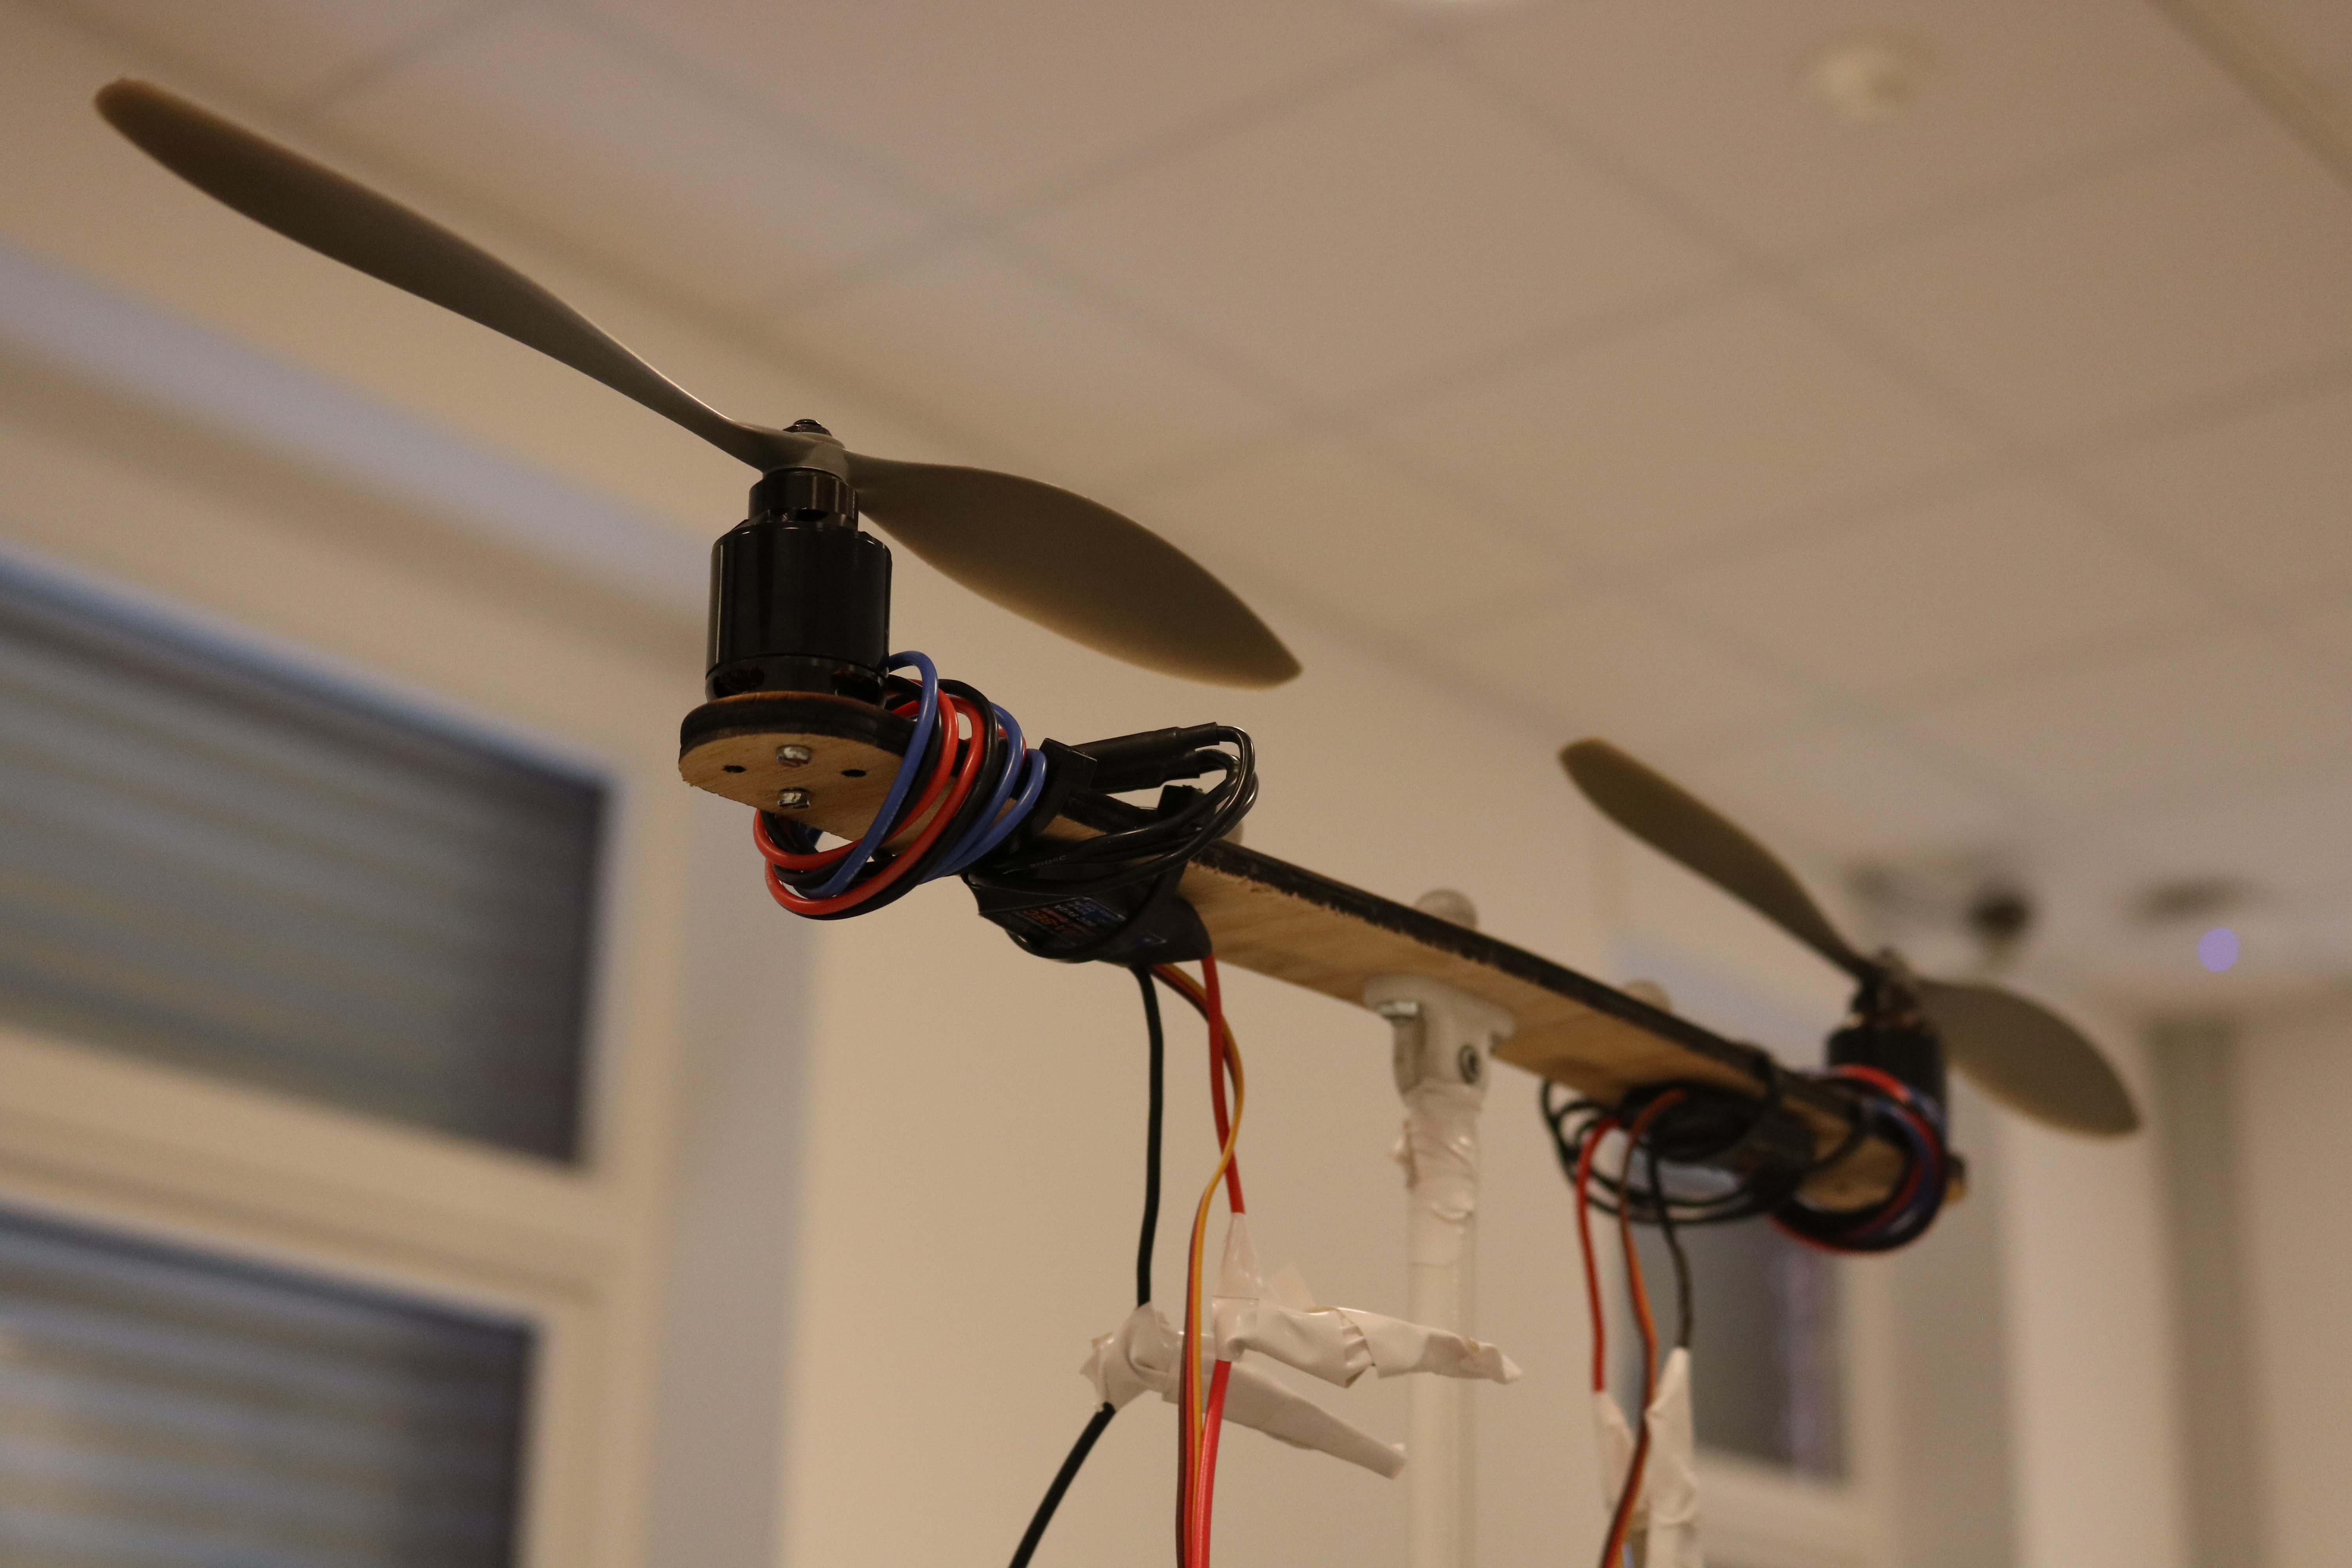
\includegraphics[width = 0.6\textwidth]{VAPIQ-PICTURES/oneaxis}
        \caption{One Axis Test Rig}
        \label{fig:oneaxis}
\end{figure}
  

\newpage
\subsection{Completion and Scope Change}

We have completed 78\% of the planned tasks and had a scope change of 16\% (Fig. \ref{fig:bds3}). The change was mainly due to the fact that the built mechanisms did not work.

Project plan status, sprint 3:

\begin{itemize}
    \item Plan Research Paper, \textbf{Started}
    \item Mechanical Design Plan, Variabel Pitch, \textbf{Started}
    \item Basic Controller, Fixed Pitch, \textbf{Started}
    \item Motor Control System, Fixed Pitch, \textbf{Started}
    \item Flight Testing And Control, \textbf{Started}
    \item Mathematical Model, Variable Pitch, \textbf{Postponed}
    \item Electrical Schematic, Fixed Pitch, \textbf{Done}
    \item Electrical Schematic, Variabe Pitch, \textbf{Done}
\end{itemize}


\begin{figure}[h]
        \centering
        \includegraphics[width = 1\textwidth]{VAPIQ-PICTURES/BDSprint3}
        \caption{Sprint 3 - Burndown Chart}
        \label{fig:bds3}
    \end{figure}
  

\subsection{Results and Conclusions}

The schematic of the components were made for both FPQ and VPQ. The team finally got stable readings from the accelerometer and looked into Quaternion based quadcopter modelling. In this sprint, the off board controller was made and started on two axis stabilization.



\begin{comment}
The mechanisms made did not work, 
    - off board flight controller
    - Started 2 axis
\subsection{Challenges}




\subsection{Lessons Learned}





\end{comment}    






